% PROJECT: <ETD> Electronic Thesis and Dissertation Initiative
%   TITLE: LaTeX report template for ETDs in LaTeX
%  AUTHOR: Neill Kipp, nkipp@vt.edu
%     URL: http://etd.vt.edu/latex/
% SAVE AS: etd.tex
% REVISED: September 6, 1997 [GMc 8/30/10]
% 

% Instructions: Remove the data from this document and replace it with your own,
% keeping the style and formatting information intact.  More instructions
% appear on the Web site listed above.

%\documentclass[12pt,dvips]{report}
\documentclass[12pt]{report}

\setlength{\textwidth}{6.5in}
\setlength{\textheight}{8.5in}
\setlength{\evensidemargin}{0in}
\setlength{\oddsidemargin}{0in}
\setlength{\topmargin}{0in}

\setlength{\parindent}{0pt}
\setlength{\parskip}{0.1in}

% Uncomment for double-spaced document.
% \renewcommand{\baselinestretch}{2}

% \usepackage{epsf}

% BHH Packages
\usepackage[]{mcode}
\usepackage[retainorgcmds]{IEEEtrantools}
\usepackage{amsmath}
\usepackage{amssymb}
\usepackage{graphicx,dblfloatfix}
\usepackage{subfig}


\begin{document}

\newcommand{\fourier}{\mathcal{F}}

\thispagestyle{empty}
\pagenumbering{roman}
\begin{center}

% TITLE
{\large
Simulation of Various Channelizer Structures 
Directed by Cyclostationary Detector}

\vfill

Brian H. Hulette

\vfill

Project Report submitted to the Faculty of the \\
Virginia Polytechnic Institute and State University \\
in partial fulfillment of the requirements for the degree of

\vfill

Master of Engineering \\
in \\
Electrical Engineering

\vfill

Amir I. Zaghloul, Co-Chair \\
Jeffrey H. Reed, Co-Chair \\
T. Charles Clancy

\vfill

February 16, 2015 \\
Falls Church, Virginia

\vfill

Keywords: SDR, Cyclostationarity, Detection, Channelizer
\\
Copyright 2015, Brian H. Hulette

\end{center}

\pagebreak

\thispagestyle{empty}
\begin{center}

{\large Simulation of Various Channelizer Structures 
Directed by Cyclostationary Detector}

\vfill

Brian H. Hulette

\vfill

(ABSTRACT)

\vfill

\end{center}

One common problem in Software-Defined Radio (SDR) systems is the problem of
detecting and then isolating narrow signals of interest in wideband sampled
data. This involves using some means to detect the frequency of one or more
signals of interest and then tuning, filtering, and decimating them. This
problem is particularly challenging due to the high sample rate of this
wideband data, so efficient algorithms are very desirable. Solutions to this
problem have applications in many areas, including both Cognitive Radio and
Electronic Warfare.

A MATLAB simulation of an SDR framework for detecting and sub-band tuning
channelized signals is presented, with a focus on finding an efficient means to
combine the two algorithms. Detection is performed using the
spectral-correlation density function which exploits the cyclostationary
property of digital signals \cite{Gardner1}.  These detections are then used to
direct a channelizer which will tune, filter, and decimate all of the detected
signals. Two different channelizer structures are examined – a polyphase
analysis/synthesis channelizer \cite{Harris1} and an overlap-save filter bank
\cite{Borgerding1}.

A summary of relevant background information is provided.  This includes
a discussion of cyclostationarity and the spectral-correlation density function
as well as background on both channelizer structures. For the overlap-save
filter bank it will be shown that in many cases computation can be saved by
using the same FFT computation for both the cyclostationary detector and the
channelizer.

In this simulation, simple QPSK signals are used to model the signals of
interest, but the framework is applicable to any modulation or signal type that
has cyclostationary features. While other means of signal detection may be more
reliable for specific signals, a cyclostationary detector's primary strength is
its ability to function for many different types of digital signals.


\vfill

% GRANT INFORMATION

%That this work received support from the Southeastern Universities
%Research Association (SURA) ``Monticello Library Project'' is purely
%coincidental.

\pagebreak

% Dedication and Acknowledgments are both optional
% \chapter*{Dedication}
\chapter*{Acknowledgments}
I would like to acknowledge the work of both Craig Carlson and Ruth Stoehr.
The core of my testbed for this project is a robust QPSK Transmitter/Receiver
pair we designed together for an ECE5654 project which we completed in the
Spring of 2013.

I would like to thank my current employer, n~ask, inc., and all of my
co-workers there for their support.

I would also like to thank the members of my committee, particularly Dr.
Zaghloul, for their patience and support.

Finally I would like to thank my friends and family, particularly my girlfriend
Meredith, for letting me use ``My Masters" as an excuse for nearly anything.

\tableofcontents
\pagebreak

\listoffigures
\pagebreak

%\listoftables
%\pagebreak

\pagenumbering{arabic}
\pagestyle{myheadings}

\chapter{Introduction}
\label{sec:intro}
\markright{Brian H. Hulette \hfill Chapter \ref{sec:intro}. Introduction \hfill}

A common problem when designing a Software-Defined Radio (SDR) system is the
problem of detecting and tuning signals of interest. A typical SDR will sample
at a relatively high rate to acquire a wideband signal. Then it will attempt to
detect the channels within the acquired frequency range that contain signals of
interest, and then tune, filter, decimate, and demodulate those signals. 

%TODO: links to SDR frameworks (webSDR) TODO: image of SDR plotting
Many popular SDR applications perform this detection step with
a "man-in-the-loop".  A falling raster of the wideband data is presented and
the man-in-the-loop will "click-tune" to select  the frequencies that (s)he
would like to process. One common version of this is to acquire a wideband
slice of the HAM radio spectrum and then click tune to different frequencies to
demodulate new FM Push-to-Talk signals and listen to them.

In this paper I will investigate and simulate a structure that automates this
process - but rather than working for a single analog signal, this framework is
intended for an arbitrary number of digital signals. Detection is performed by
a cyclostationary detector rather than by a man-in-the-loop, in order to
exploit the cyclostationary properties exhibited by most digital signals with
a fixed symbol rate.  Tuning, filtering, and decimating is performed by
a channelizer, so that many signals can be processed at once.  I will examine
two different channelizer structures. They will be compared on two important
criteria:
1) Their ability to accurately reproduce every detected signal, and 2) Their
computational efficiency when combined with a cyclostationary detector.
% TODO: list papers that discuss SCD for various protocols

In Chapter~\ref{sec:cyclo} I will provide background information on
cyclostationary properties and the cyclic spectra upon which my detector
relies.  Chapter~\ref{sec:chan} discusses and compares both of the channelizer
structures that I will simulate. Chapter~\ref{sec:sim}  discusses the MATLAB
simulation I have created and the results of it. Finally,
Appendix~\ref{sec:source} provides annotated source code for key parts of the
simulation, as well as locations where the entire source code can be found.

\chapter{Cyclostationary Detection}
\label{sec:cyclo}
\markright{Brian H. Hulette \hfill Chapter \ref{sec:cyclo}. Cyclostationary Detection \hfill}

\section{Cyclostationarity}
\label{sec:cyclo_prop}
Often signals are modeled as stochastic random processes with properties such as
mean and variance, but many man-made signals, particularly digital communications,
can be modeled with another statistical property called
\emph{cyclostationarity} which implies the signal has some parameter which
varies with time. The frequency of this variation is called the cyclic
frequency, $\alpha$. \cite{Gardner1}.


Of particular interest is second-order cyclostationarity, where a signal has a
periodic autocorrelation:

\begin{IEEEeqnarray*}{lCl}
    R_{xx}(t, t+\tau) = E\{x(t)x^*(t+\tau)\} = \sum_{\alpha} R_{xx}^{\alpha}(\tau)e^{j2 \pi \alpha t}
\end{IEEEeqnarray*}

% TODO more detail here based on Oner1

\begin{IEEEeqnarray*}{lCl}
    R_{xx}^{\alpha}(\tau) = \lim_{T \to \infty} \frac{1}{T}\int_{-T/2}^{T/2} R_{xx}(t, t+\tau)e^{-j2\pi \alpha t} dt
\end{IEEEeqnarray*}
% TODO: reference papers that perform time domain detection (listed in "Energy Efficient Spectrum Sensing using Cyclostationarity")
% "Cyclostationary Based Air Interface Recognition For Software Radio Systems" is also a time domain approach
The cyclic autocorrelation function (CAF), given by $R_{xx}^{\alpha}(\tau)$,
can be used for signal detection in the time domain. An estimate of the 2D
function versus $\alpha$ and $\tau$ can be computed, then features within this
plane can be detected. However, what I am interested in is the fourier
transform of the CAF, called the Spectral Correlation Density (SCD):

\begin{IEEEeqnarray*}{lCl}
    S_{xx}(\alpha, f) = \int_{-\infty}^{\infty} R_{xx}^{\alpha}(\tau)e^{-j2\pi f \tau} d\tau
\end{IEEEeqnarray*}

The SCD is a generalization of the conventional PSD, which it reduces to at
$\alpha=0$ \cite{Oner1}. Like the CAF, the SCD also contains unique features
based on the modulation type, symbol rate, and carrier frequency of the
transmitted signal, which we can exploit for signal detection. In
\cite{Gardner2}, Gardner defines this SCD for various basic modulation types,
including QPSK, which is used in my simulation.

%\section{Exploiting Cyclostationarity for Detection}
%\label{sec:exploit_cyc}
%For the problem defined in Chapter \ref{sec:intro} we can define the wideband
%signal $W(t)$ as the sum of $N$ cyclostationary signals, tuned to
%various frequencies, in an AWGN channel:
%\begin{IEEEeqnarray*}{lCl}
%    W(t) & = & \sum C_{i}(t) e^{j 2 \pi f_i t} + N(t)
%\end{IEEEeqnarray*}
%
%Where the $C_i(t)$ are cyclostationary random processes at various symbol rates,
%tuned to corresponding frequencies $f_i$ and $N(t)$ is the AWGN.
%
%We would like to exploit the cyclostationarity of the $C_i$ waveforms to
%identify the frequency, $f_i$, of those waveforms which are transmitted at a
%specific symbol rate.

\section{Estimating the SCD}
% Use Gardner1 to show that SCD is conjugate multiplication of frequency shifted spectra
% TODO:
% - cyclic wiener relation on Gardner1 pg. 153
% - attempts to derive in lab notebook pg. 20-21
Thus we can compute a discrete slice of the SCD at cyclic freqency $\alpha$ as
the cross spectral density of the two frequency-shifted time sequences
$x_L(t) = x(t)e^{j\pi\alpha t}$ and $x_U(t) = x(t)e^{-j\pi\alpha t}$. The cross
spectral density of these two sequences is equivalent to the conjugate
multiplication of their individual fourier transforms:

\begin{IEEEeqnarray*}{lCl}
    S_{xx}(\alpha, f) & = & X_L(f)X_U^* (f) \\
                      & = & X(f - \alpha/2)X^*(f + \alpha/2)
\end{IEEEeqnarray*}

% Discuss possibility of circular shifting a forward FFT to estimate SCD slice
This means that we can compute $S_{xx}(\alpha, f)$ using a single forward FFT
by shifting the spectrum in either direction by $\alpha/2$, and then conjugate
multiplying the two shifted spectra together. This is significant, since
a simple forward FFT of the acquired data is useful for other operations, such
as channelization, as we will see in Section \ref{sec:poly_chan}.

Of course there is a caveat. In order to perform this shift accurately using an
FFT we need to circular shift the FFT by an integer number of bins.  This
means we can only accurately perform this frequency shift when $\alpha/2$ is
a multiple of the FFT resolution.  Thus $\alpha$ must satisfy the following
relationship:
\begin{IEEEeqnarray*}{lCl}
    \alpha = \frac{2kf_s}{N_{fft}} \text{, } k \in \mathbb{Z}
\end{IEEEeqnarray*}

If an estimate of the SCD at a cyclic frequency that does not satisfy this
relation is required, then we must perform the frequency shift in the time
domain to be perfectly accurate. Alternatively, we can still use a single
forward FFT and approximate the shift by interpolating between bins, but this
is only an approximation.


\chapter{Channelizer Structures}
\label{sec:chan}
\markright{Brian H. Hulette \hfill Chapter \ref{sec:chan}. Channelizer Structures\hfill}
\section{Polyphase Analysis/Synthesis Channelizer}
\label{sec:poly_chan}
Fred Harris has described the related structures that he calls Polyphase
Analysis and Polyphase Synthesis Channelizers \cite{Harris1}. A Polyphase
Analysis channelizer can be used to break up a wideband signal into $N$ distinct
channels, each decimated by a factor of $N$ from the wideband sample rate. The
channelized frequencies are integer multiples of the output sample rate:

\begin{IEEEeqnarray}{lCl}
    f_k = k \frac{f_s}{N}
\end{IEEEeqnarray}

Where $f_k$ is the center frequency of channel $k$ and $f_s$ is the input sample
rate. A Polyphase Synthesis Channelizer performs the reverse operation - it
combines $N$ distinct channels with equal sample rate into a single wideband
signal.

These two structures can be combined to create a very flexible channelizer that
can tune channels with arbitrary center frequencies and various bandwidths
\cite{Harris2}.

In \cite{Harris1}, Harris shows how the Polyphase Analysis Channelizer works by
starting with a basic filter/decimator and making incremental modifications
until it becomes an Analysis Channelizer as shown in Figure
\ref{fig:polyphase_4}. I will provide a brief summary of this description here.


\begin{figure}[h!]
\centerline{
    \subfloat[Single channel of a simple tuning, filtering, and decimating channelizer. $h(n)$ is a baseband low-pass filter.]
    {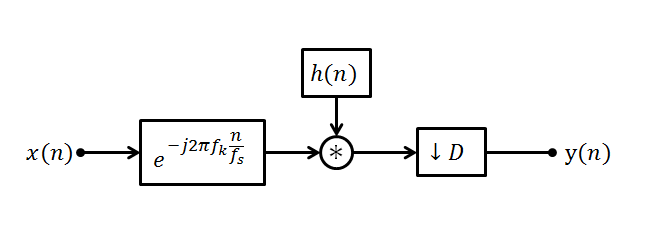
\includegraphics[width=0.45\textwidth]{polyphase_1}%
    \label{fig:polyphase_1}}
    \hfill
    \subfloat[Equivalency theorem allows the tuning step to be moved after the decimation. The baseband filter must be shifted up to $f_k$. If $f_k$ is a multiple of the output sample rate,  $\frac{f_s}{D}$, the tuning step can be dropped.]
    {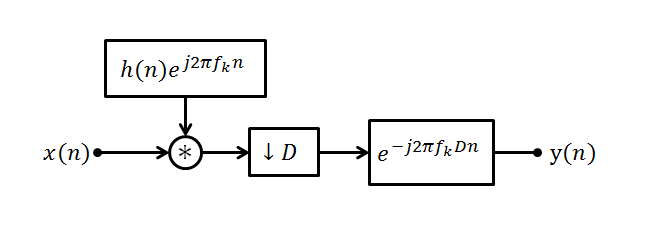
\includegraphics[width=0.45\textwidth]{polyphase_2}%
    \label{fig:polyphase_2}}
}
\centerline{
    \subfloat[The Noble Identity allows the filtering and decimation to be combined to remove excess computations.]
    {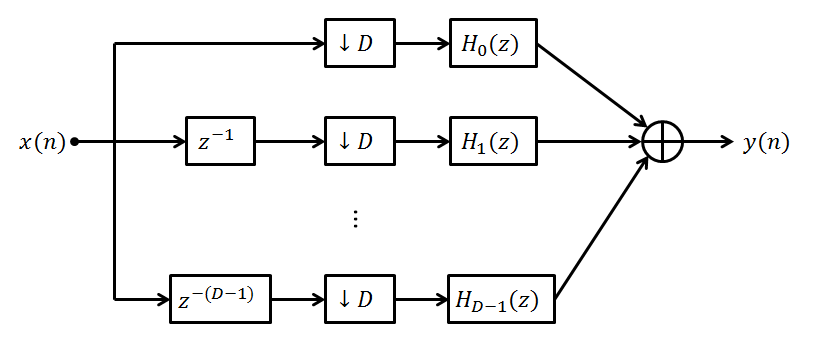
\includegraphics[width=0.45\textwidth]{polyphase_3}%
    \label{fig:polyphase_3}}
    \hfill
    \subfloat[The series of delays and decimation steps can be replaced with an input commutator and complex phasors can be added after each filter to select channel $k$.]
    {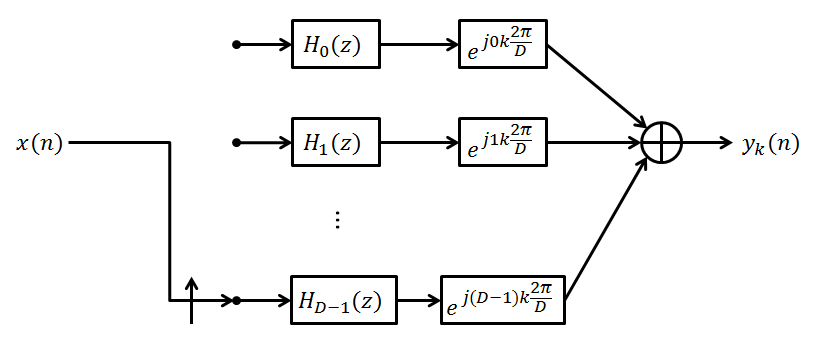
\includegraphics[width=0.45\textwidth]{polyphase_4}%
    \label{fig:polyphase_4}}
}
\caption{Creating a single channel of a polyphase analysis channelizer}
\label{fig:polyphase_proof}
\end{figure}

We start with a single channel of a very basic channelizer in Figure
\ref{fig:polyphase_1}. This channel consists of a multiplication with a complex
phasor to tune the desired center frequency down to baseband, followed by
a low-pass filter, represented by $h(n)$, and finally a decimation step. The
first modification we can make takes advantage of the Equivalency Theorem,
which says that we can switch the order of the tuner and the filter, \emph{if}
the filter is changed to a bandpass filter centered at $f_k$. This modification
is shown in Figure \ref{fig:polyphase_2}. In this figure the tuner has also
been moved after the decimator. Note that if the channel frequency, $f_k$, is
an integer multiple of the output sample rate, $\frac{f_s}{D}$, then the tuner
simplifies to $e^{j2\pi n} = 1$, so it can be dropped completely.  Thus we will
restrict the polyphase analysis channelizer to center frequencies which are
integer multiples of the output sample rate.

Next we can use the Noble Identity to switch the place of the decimation and
the filter, as shown in Figure \ref{fig:polyphase_3}. In order to do so we need to define a set of new filters, $H_r(z)$, such that:

\begin{IEEEeqnarray}{lCl}
    H(z) = H_0(z^D) + z^{-1}H_1(z^D) + \hdots + z^{-(D-1)}H_{D-1}(z^D)
\end{IEEEeqnarray}

This means that each filter, $H_r(z)$, has has an impulse response which is $h(n)$
shifted by $r$ samples and decimated by $D$. Using the Noble Identity in this
way saves us from performing computations for samples that will just be dropped
by the decimator. Note that in Figure \ref{fig:polyphase_3} the tuner has been
dropped since we are restricting the channelizer to frequencies which are
multiples of the output sample rate.

Finally, we complete the structure for a single channel of a polyphase analysis
channelizer in Figure \ref{fig:polyphase_4}. The combination of delays and
decimators at the front of the previous structure is actually just
a commutator. In \cite{Harris1} Harris explains this by thinking about the
decimators as a switch that closes every $D$ samples. So in Figure
\ref{fig:polyphase_3}, when all of the switches close the filter at the bottom
gets the oldest sample, and each filter as you go up gets one newer sample
until you get to the most recent sample on the top. The next sample is not
processed until the switches close again, and it is passed to the filter at the
bottom. With this explanation it is easy to see the whole structure can be
replaced with a commutator.

The final structure has one more modification. The outputs are multiplied by complex phasors which select the individual channel, $k$, centered at $f_k$. For more info on why this works refer to \cite{Harris1}. The great thing about these complex phasors is that the set of phasors that are multiplied and then summed together for channel $k$ correspond to the $k$th output of a DFT:

\begin{IEEEeqnarray}{lCl}
    y_k(n) & = & \sum_{r=0}^{D-1} y_r(n) e^{j(2\pi/D)rk} 
\end{IEEEeqnarray}

Where $y_r(n)$ represents the output of filter $H_r(z)$. Thus we can compute
all $D$ channels using a $D$ point FFT, as shown in Figure
\ref{fig:polyphase_final}. The structure of the Polyphase Synthesis Channelizer
can be seen in Figure \ref{fig:polyphase_synthesis}. It is essentially a mirror
image of the Analysis case - an IFFT followed by filters and a reverse
commutator.

% TODO: reverse commutator? is that a thing?

\begin{figure}[h!]
\centerline{
    \subfloat[Analysis]
    {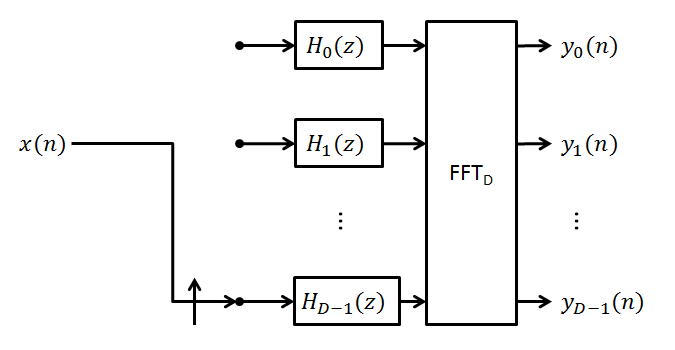
\includegraphics[width=0.45\textwidth]{polyphase_final}%
    \label{fig:polyphase_final}}
    \hfill
    \subfloat[Synthesis]
    {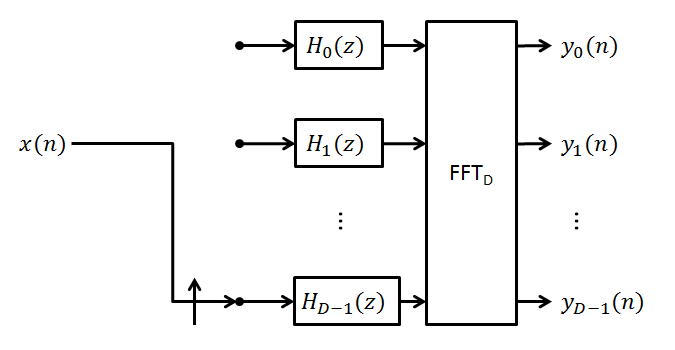
\includegraphics[width=0.45\textwidth]{polyphase_final}%
    \label{fig:polyphase_synthesis}}
}
\caption{Full Polyphase Analysis/Synthesis Channelizer Structures}
\label{fig:overlap_save_filter_banks}
\end{figure}

\subsection{Limitations}
\label{sec:poly_limitations}
This structure has a couple of obvious limitations if a Polyphase Analysis
Channelizer is used by itself. Every channel must be at the same output sample
rate, $f_s/D$, and they must have center frequencies which are multiples of
that sample rate.

In \cite{Harris2}, Harris shows how analysis and synthesis
channelizers can be used in concert, along with complex phasors, to tune out
arbitrary center frequencies at unequal sample rates. Unfortunately, this adds
a significant amount of complexity and is beyond the scope of this project.

\subsection{Advantages}
\label{sec:poly_advantages}
The primary advantage of a Polyphase Analysis Channelizer is its simplicity and efficiency.

\section{Overlap-save Filter Bank}
\label{sec:filter_bank}
The ``overlap-save filter bank" structure that I use is based entirely on
a description by Mark Borgerding from March 2006 \cite{Borgerding1}.
Borgerding's concept is based on the well known Overlap-Save fast convolution
technique.

% TODO cite Borgerdings [1]-[5] here for Overlap-Save?
OS fast convolution can be used to speed up convolution with
a filter that has a long impulse response. The concept is that rather than
convolving in the time-domain - complexity $O(N^2)$ - it is faster to first
perform an FFT of both the signal and the filter and multiply in the frequency
domain, then IFFT to go back to the time domain - complexity $O(N\log_2N)$.
There is nothing new about this idea, but Borgerding's innovation is that he
shows how to extend this concept to tune, filter and decimate any number of
channels with arbitrary frequencies and bandwidths.

For my description, I will use the same terms that Borgerding defines:

\begin{tabular}{ll}
    $x(n)$        & Input data \\
    $h(n)$        & Baseband filter response \\
    $y(n)$        & Tuned, filtered and decimated output data \\
    $P$           & Length of $h(n)$ \\
    $N$           & FFT size \\
    $D$           & Decimation factor \\
    $V = N/(P-1)$ & Ratio of FFT size to filter order \\
\end{tabular}

\begin{figure}[h!]
\centerline{
    \subfloat[Performing frequency shift by circular shifting the FFT output]
    {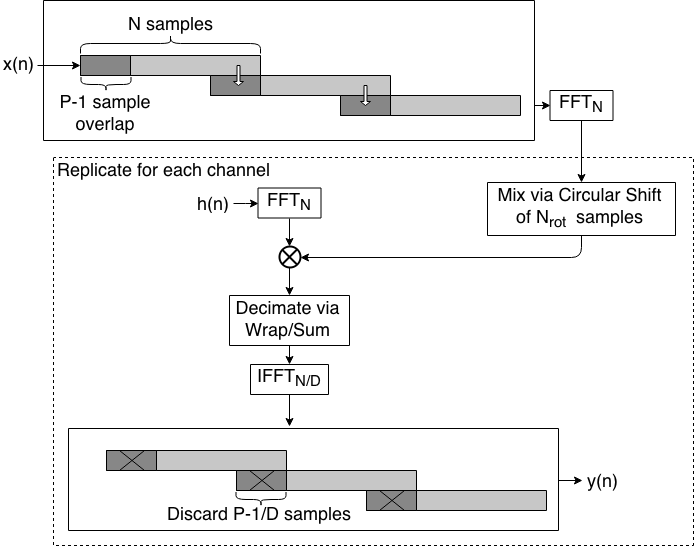
\includegraphics[width=0.45\textwidth]{overlap_save_shift}%
    \label{fig:overlap_save_shift}}
    \hfill
    \subfloat[Performing precise frequency shift in the time-domain]
    {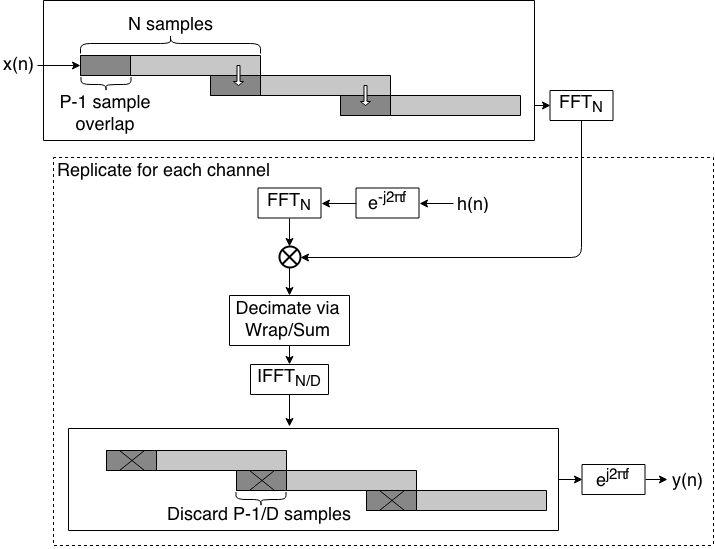
\includegraphics[width=0.45\textwidth]{overlap_save_time_domain}%
    \label{fig:overlap_save_time_domain}}
}
\caption{Overlap-Save Filter Bank Structures}
\label{fig:overlap_save_filter_banks}
\end{figure}

\emph{Tuning:} If the frequency of the signal of interest corresponds to one of
the FFT bins then we can simply circular shift the FFT output to place that bin
at the center. Then filtering can be performed at baseband.  If all channels
satisfy this criteria then we can re-use a single forward FFT for every
channel, simply by circular shifting it to the appropriate bin in every case. 
This approach is shown in Figure \ref{fig:overlap_save_shift}

However, if this condition is not satisfied then we will need to perform the
frequency shift in the time domain by multiplying by a complex phasor.
Fortunately, there is a still a way to re-use the forward FFT in this case.
After taking an FFT of the non frequency-shifted signal we can shift the
baseband filter response up to the desired frequency, then after the filtered
signal is IFFT'd back into the time domain, we perform the frequency shift with
a complex phasor.  This is even better than frequency shifting before the
forward FFT since the multiplication is performed after decimation. This
approach is shown in Figure \ref{fig:overlap_save_time_domain}.

\emph{Decimation:} Following the frequency domain filtering we have two
different options for decimation. The first option is to perform a full size
inverse FFT of the output, and then decimate in the time domain. The issue with
this approach is that we are computing a larger inverse FFT than we really need
to. As a solution to this, Borgerding suggests decimating in the frequency
domain. The approach (called ``Wrap/Sum" in Figure
\ref{fig:overlap_save_filter_banks}) is simple: coherently add together the aliased
components of the frequency spectrum.  For example, if the FFT size is 1024 and
we need to decimate by a factor of 4, then coherently sum FFT samples 0 to 255,
256 to 511, 512 to 767 and 768 to 1024.  The result is a 256 sample frequency
spectrum which we can now inverse FFT to produce the decimated output. The only
trick with this approach is that we must discard just $(P-1)/D$ samples rather
than $P-1$ to accont for the overlap.  This reveals one restriction of this
structure: the filter order $P-1$ must be an integer multiple of the
decimation, $D$.

\subsection{Limitations}
\label{sec:os_limitations}
There are a few limitations of this structure that are worth mentioning. First,
as mentioned earlier, the filter order $P-1$ must be an integer multiple of the
decimation factor $D$. This problem is pretty easy to solve though, simply
zero-pad the filter to achieve an appropriate length. Another limitation that
is potentially challenging is that the FFT size, $N$, must be an integer
multiple of the decimation rate, $D$. So decimation rates whose prime factors
are larger than 2 or 5 (or others, depending on the FFT implementation) could
lead to FFT inefficency for this structure.

One more limitation occurs when attempting to rotate the FFT to frequency shift.
As previously mentioned, the precision of the frequency shift is limited by the
resolution of the FFT. However, the precision is also limited further by the
ratio of FFT size to filter order, $V$. This is because we must restrict mixing
to the frequencies whose period completes in $L=N-(P-1)$ samples. Borgerding
provides the following equation for computing the number of FFT bins to rotate
to shift to frequency $f$ (\cite{Borgerding1} Equation (1)):

\begin{equation*}
    N_{rot} = \text{round}\left( \frac{Nf}{Vf_s} \right) V
\end{equation*}

Where $f_s$ is the base sample rate. This equation simply adjusts $N_{rot}$ to
the nearest multiple of $V$ bins. It is worth noting that my solution for
making $P-1$ an integer multiple of $D$ is only making this problem worse by
making $V$ larger - but there's nothing to be done about that other than opting
for a shorter filter.

\subsection{Advantages}
\label{sec:os_scd_estimation}

The greatest benefit of the Overlap-Save Filter Bank for my application is
the ease with which it can be combined with SCD Estimation for cyclostationary
detection. Obviously, the first step for both algorithms is a forward FFT of the
wideband input. If we were to design a joint cyclostationary
detector/Overlap-Save Filter Bank we could re-use the same forward FFT for both
algorithms.

The only design challenge (which is certainly significant) is finding
a combination of FFT size, sample rate, and decimation factor that will work
for both algorithms.

% TODO: Analysis of this problem. Decimation factor is related to alpha by the amount of oversampling.
% Started this analysis a bit in lab notebook pg. 23

%We can say that the output sample rate is some integer multiple of the symbol rate:
%\begin{equation}
%    f_s' = \beta \alpha \text{, } \beta = 1,2,\hdots
%\end{equation}
%Where the integer multiple $\beta$ is simply the amount of oversampling. Then we can 

Averaging the overlapped FFT frames together may have an effect on the accuracy
of the SCD estimation, but analyzing this effect is beyond the scope of this
project.

\chapter{Simulation}
\label{sec:sim}
\markright{Brian H. Hulette \hfill Chapter \ref{sec:sim}. Simulation \hfill}
I have created a MATLAB simulation of these structures. Directions to find all
of the source code can be found in Appendix \ref{sec:source}. Each module
- cyclostationary detector, polyphase analysis channelizer, and overlap-save
filter bank - was developed and tested separately. I then combined the detector
with each channelizer and evaluated their performance. I will follow that same
logical flow in this Chapter as I describe the simulation.

\section{Cyclostationary Detector}
\label{sec:sim_cyclo}

\section{Polyphase Analysis Channelizer}
\label{sec:sim_poly}

\subsection{Adding Cyclo Detection}
\label{sec:sim_poly_cyclo}

\section{Overlap-Save Filter Bank}
\label{sec:sim_os}

\subsection{Adding Cyclo Detection}
\label{sec:sim_os_cyclo}

\chapter{Conclusion}
\label{sec:conclusion}
\markright{Brian H. Hulette \hfill Chapter \ref{sec:conclusion}. Conclusion \hfill}

%%%%%%%%%%%%%%%%%
%
% Include an EPS figure with this command:
%   \epsffile{filename.eps}
%

%%%%%%%%%%%%%%%%
%
% Do tables like this:

% \begin{table}
% \caption{The Graduate School wants captions above the tables.}
%\begin{center}
% \begin{tabular}{ccc}
% x & 1 & 2 \\ \hline
% 1 & 1 & 2 \\
% 2 & 2 & 4 \\ \hline
% \end{tabular}
%\end{center}
% \end{table}

%%%%%%%%%%%%%%%%%%%%%%%%%%%%%%%%

% If you are using BibTeX, uncomment the following:
\nocite{*}
\bibliographystyle{IEEEtran}
\bibliography{bibliography}
%
% Otherwise, uncomment the following:
% \chapter*{Bibliography}

\appendix

% In LaTeX, each appendix is a "chapter"
\chapter{Project Source}
\label{sec:source}
\markright{Brian H. Hulette \hfill Chapter \ref{sec:source}. Project Source \hfill}
% TODO: make sure this is a link - and make the project public!
The full source is hosted on GitHub
(\texttt{https://github.com/TheNeuralBit/cyclo\_channelizer}). Some of the
critical files are included in this appendix.

\section{\texttt{cyclic\_spectrum.m}}
\lstinputlisting{../cyclo/cyclic_spectrum.m}
\section{\texttt{synthesis\_channelizer.m}}
\lstinputlisting{../synthesis_channelizer.m}
\section{\texttt{analysis\_channelizer.m}}
\lstinputlisting{../analysis_channelizer.m}
\section{\texttt{overlap\_save\_channelizer.m}}
\lstinputlisting{../overlap_save_channelizer.m}

\end{document}
